
\chapter{Examples}
\label{chap:examples}

\section{teste}
\subsection{teste}
\subsubsection{teste}

% \tikzset{
%  every node/.style={font=\tiny},
%     }
% \KOMAoptions{paper=a3,paper=landscape}
% \recalctypearea

% \begin{figure}[H]
% \vspace{-2cm}
% \centerline{\includegraphics[height=1.28\textheight]{../../data/stdin}}
% % \centerline{\resizebox{!}{1.2\textheight}{\begin{tikzpicture}[>=latex',line join=bevel,]
%%
\begin{scope}
  \pgfsetstrokecolor{black}
  \definecolor{strokecol}{rgb}{1.0,1.0,1.0};
  \pgfsetstrokecolor{strokecol}
  \definecolor{fillcol}{rgb}{1.0,1.0,1.0};
  \pgfsetfillcolor{fillcol}
\end{scope}
  \node (x13) at (820.63bp,204.75bp) [draw,circle, double,place, label=above:,rotate=0] {$x_{13}$};
  \node (x12) at (623.63bp,229.75bp) [draw,,circle, label=above:,rotate=0] {$x_{12}$};
  \node (x8) at (623.63bp,531.75bp) [draw,circle, double,place, label=above:,rotate=0] {$x_{8}$};
  \node (x2) at (413.63bp,294.75bp) [draw,,circle, label=above:,rotate=0] {$x_{2}$};
  \coordinate (init) at (28.63bp,208.75bp);
  \node (x9) at (190.63bp,75.748bp) [draw,,circle, label=above:,rotate=0] {$x_{9}$};
  \node (x11) at (518.63bp,229.75bp) [draw,,circle, label=above:,rotate=0] {$x_{11}$};
  \node (x10) at (302.63bp,75.748bp) [draw,circle, double,place, label=above:,rotate=0] {$x_{10}$};
  \node (x3) at (518.63bp,363.75bp) [draw,,circle, label=above:,rotate=0] {$x_{3}$};
  \node (x0) at (93.63bp,208.75bp) [draw,,circle, label=above:,rotate=0] {$x_{0}$};
  \node (x1) at (242.63bp,358.75bp) [draw,,circle, label=above:,rotate=0] {$x_{1}$};
  \node (x6) at (190.63bp,208.75bp) [draw,,circle, label=above:,rotate=0] {$x_{6}$};
  \node (x7) at (302.63bp,234.75bp) [draw,,circle, label=above:,rotate=0] {$x_{7}$};
  \node (x4) at (715.63bp,290.75bp) [draw,,circle, label=above:,rotate=0] {$x_{4}$};
  \node (x5) at (820.63bp,376.75bp) [draw,circle, double,place, label=above:,rotate=0] {$x_{5}$};
  \draw [-Latex] (x4) ..controls (740.45bp,270.42bp) and (776.04bp,241.27bp)  .. (x13);
  \definecolor{strokecol}{rgb}{0.0,0.0,0.0};
  \pgfsetstrokecolor{strokecol}
  \draw (763.63bp,274.25bp) node {\scriptsize $\uparrow$1$\uparrow$2$\downarrow$3 \{3\}};
  \draw [-Latex] (x2) ..controls (440.38bp,278.19bp) and (476.09bp,256.08bp)  .. (x11);
  \draw (464.63bp,284.25bp) node {\scriptsize $\uparrow$1 \{3\}};
  \draw [-Latex] (x0) ..controls (125.39bp,240.72bp) and (195.71bp,311.52bp)  .. (x1);
  \draw (142.63bp,286.25bp) node {\scriptsize $\uparrow$2 \{0\}};
  \draw [-Latex] (x11) ..controls (549.13bp,229.75bp) and (579.37bp,229.75bp)  .. (x12);
  \draw (569.63bp,239.25bp) node {\scriptsize $\downarrow$1$\downarrow$2$\downarrow$3 \{3\}};
  \draw [-Latex] (x6) ..controls (219.89bp,215.54bp) and (258.12bp,224.42bp)  .. (x7);
  \draw (242.63bp,234.25bp) node {\scriptsize $\uparrow$1$\uparrow$2 \{1, 3\}};
  \draw [-Latex] (x1) ..controls (280.92bp,344.42bp) and (357.34bp,315.82bp)  .. (x2);
  \draw (302.63bp,351.25bp) node {\scriptsize $\downarrow$1$\uparrow$3 \{0\}};
  \draw [-Latex] (x0) ..controls (120.39bp,208.75bp) and (149.16bp,208.75bp)  .. (x6);
  \draw (142.63bp,218.25bp) node {\scriptsize $\downarrow$1 \{1, 3\}};
  \draw [-Latex] (init) ..controls (58.462bp,208.75bp) and (65.783bp,208.75bp)  .. (x0);
  \draw [-Latex] (x2) ..controls (440.34bp,312.3bp) and (478.01bp,337.06bp)  .. (x3);
  \draw (464.63bp,350.25bp) node {\scriptsize $\downarrow$2$\downarrow$3 \{0, 1\}};
  \draw [-Latex] (x3) ..controls (540.89bp,399.37bp) and (586.69bp,472.65bp)  .. (x8);
  \draw (569.63bp,481.25bp) node {\scriptsize $\uparrow$1 \{1\}};
  \draw [-Latex] (x12) ..controls (650.18bp,247.35bp) and (679.13bp,266.55bp)  .. (x4);
  \draw (672.63bp,280.25bp) node {\scriptsize $\uparrow$3 \{3\}};
  \draw [-Latex] (x4) ..controls (740.8bp,311.36bp) and (777.58bp,341.49bp)  .. (x5);
  \draw (763.63bp,353.25bp) node {\scriptsize $\uparrow$1$\downarrow$3 \{0\}};
  \draw [-Latex] (x9) ..controls (218.67bp,75.748bp) and (251.27bp,75.748bp)  .. (x10);
  \draw (242.63bp,85.248bp) node {\scriptsize $\uparrow$1$\downarrow$2$\downarrow$3 \{2\}};
  \draw [-Latex] (x7) ..controls (330.95bp,250.05bp) and (371.05bp,271.73bp)  .. (x2);
  \draw (361.63bp,286.25bp) node {\scriptsize $\downarrow$1$\uparrow$3 \{1, 3\}};
  \draw [-Latex] (x3) ..controls (560.69bp,348.16bp) and (653.99bp,313.59bp)  .. (x4);
  \draw (623.63bp,338.25bp) node {\scriptsize $\uparrow$3 \{0\}};
  \draw [-Latex] (x0) ..controls (116.29bp,177.68bp) and (157.03bp,121.81bp)  .. (x9);
  \draw (142.63bp,175.25bp) node {\scriptsize $\downarrow$1$\uparrow$2$\uparrow$3 \{2\}};
%
\end{tikzpicture}
}}
% \end{figure}

% \KOMAoptions{paper=a4,paper=portrait}
% \recalctypearea

% \addtikzfigure{../../data/stdin}
% {Petri net of Initialization module.}
% {petriinitialization}

% \begin{figure}[H]
%   \centering
%   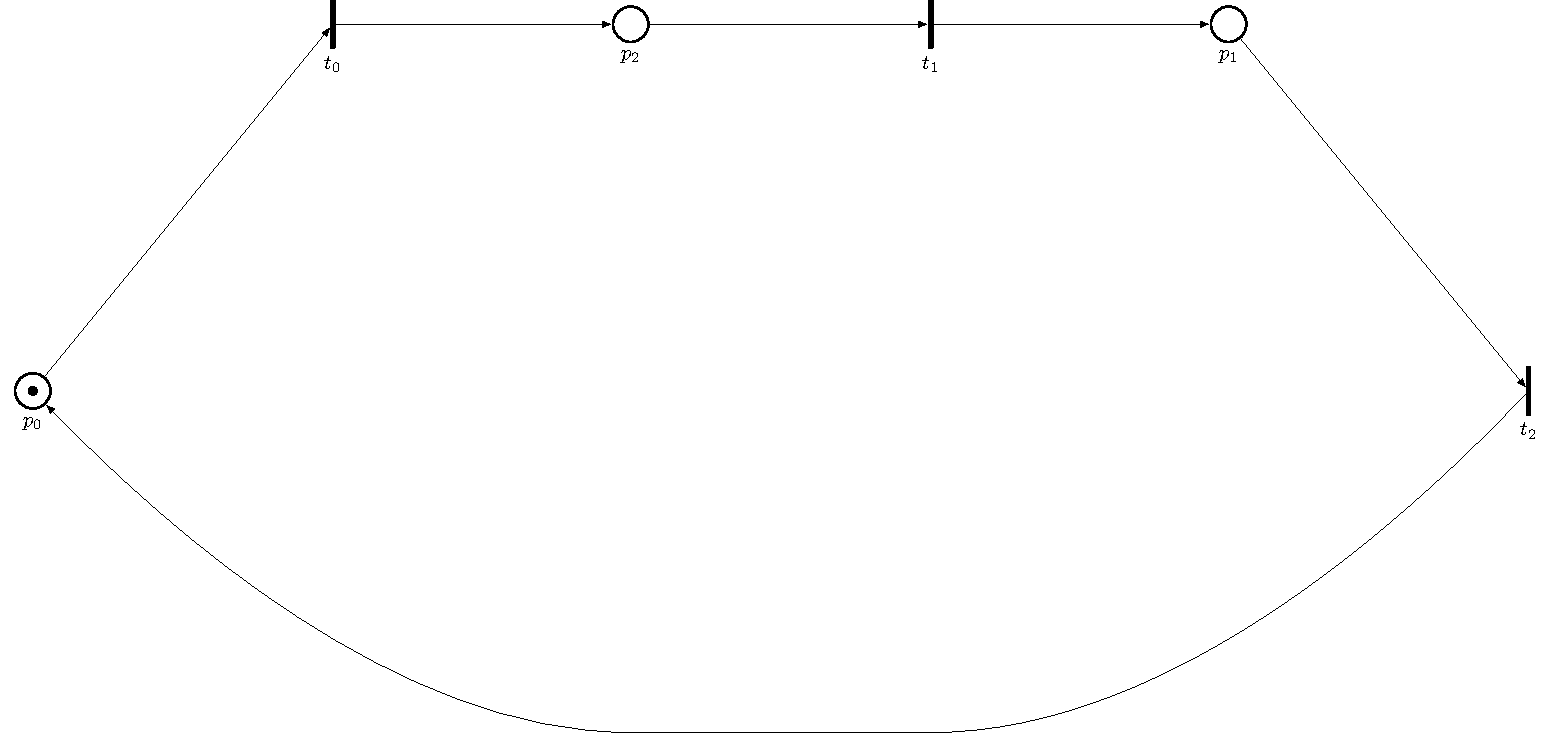
\includegraphics[width=8cm]{/home/accacio/Downloads/lixo/teste}
%   \caption{bla}
% \end{figure}


%%% Local Variables:
%%% mode: latex
%%% TeX-master: "../monografia"
%%% End:
